\section{The Kinematics-Aware Latent World Models}
\label{03_greedy_algorithm}

This section provides a detailed introduction to our proposed kinematics aware world model, which integrates multi-modal encoding, RSSM-based dynamics with driving-specific supervision, and latent-space policy learning to enable data-efficient training with explicit driving semantics.

\subsection{Multi-modal Encoding}
To address the limitations of pure image input, we propose an enhanced input representation that fuses image features with 5-dimensional vehicle physical information. These physical states can be accurately and efficiently obtained from onboard sensors (e.g., IMU, odometry), offering a reliable and low-cost alternative to inferring them from pixels.

Specifically, the image encoder processes the front-facing camera image \( I_t \) through a convolutional neural network (CNN):\( f_{\text{img}} = \text{CNN}(I_t; \theta_{\text{img}}) \). The physics encoder processes the normalized vehicle physics vector \( v_t \) through a multi-layer perceptron (MLP): \( f_{\text{phys}}= \text{MLP}(v_t; \theta_{\text{phys}}) \). Finally, the visual and physics features are concatenated to form the unified observation embedding:
\begin{equation}
e_t = \text{Concat}(f_{\text{img}}, f_{\text{phys}}) \in \mathbb{R}^{d_{\text{img}} + d_{\text{phys}}}.
\end{equation}

By incorporating this information explicitly, the world model does not have to infer dynamics solely from visual observations, allowing it to focus on learning environmental dynamics and interactions.

\subsection{Latent Dynamics Modeling}
The encoded observations embedding is then fed into a Recurrent State-Space Model (RSSM)\cite{hafner2025mastering}. At each time step, the model maintains a deterministic hidden state $h_t$ that summarizes past information, and a stochastic state $z_t$ that captures uncertainty. The transition is defined as:
\begin{equation}
\begin{aligned}
&h_t = f_\theta(h_{t-1}, z_{t-1}, a_{t-1}), \\
&\text{Prior: } \hat{z}_t \sim p_\theta(\hat{z}_t \mid h_t), \\
&\text{Posterior: } z_t \sim q_\theta(z_t \mid h_t, e_t),
\end{aligned}
\end{equation}
where $f_\theta$ is a recurrent neural network. $z_t$ is sampled from the posterior distribution during training, and prior distribution during inference. $(h_{t}, z_{t})$ together form the latent state. 

The basic world model loss consists of prediction loss and KL regularization loss:
\begin{equation}
\mathcal{L}_{\text{basic}} = \mathbb{E}_{q_\theta}\left[\sum_{t=1}^{T} \left(\mathcal{L}_{\text{pred},t} + \mathcal{L}_{\text{KL},t}\right)\right],
\end{equation}
where $\mathcal{L}_{\text{pred},t}$ includes the negative log-likelihood of observation reconstruction $-\ln p_\theta(\hat{o}_t \mid h_t, z_t)$, reward prediction $-\ln p_\theta(\hat{r}_t \mid h_t, z_t)$, and termination signal prediction $-\ln p_\theta(\hat{c}_t \mid h_t, z_t)$. The $\mathcal{L}_{\text{KL}, t} = D_{\text{KL}}(q_\theta(z_t \mid h_t, e_t) \parallel p_\theta(\hat{z}_t \mid h_t))$ is the KL divergence between the posterior and prior distribution, constraining the encoder to avoid extracting irrelevant information from observations and enhancing the consistency and predictability of the latent state.

\subsection{Driving-Specific Supervision Heads}
Relying solely on pixel reconstruction often neglects structured semantic information and cannot guarantee geometric consistency required for long-horizon interaction prediction, as critical driving elements such as lane boundaries and surrounding vehicles occupy only a small fraction of the visual input. We extend the output heads of the basic world model by adding two task-specific detection heads. The gradients of these two new heads are backpropagated to the world model, guiding the latent state to explicitly focus on key driving scene information.

A Lane Detection Head is designed to predict key lane-related information from the latent state, which are three critical indicators for lane keeping in autonomous driving: 
\begin{equation}
\hat{l}_t = f_{\text{lane}}(h_t,z_t) = \left[\hat{d}_{\text{left}}, \hat{d}_{\text{right}}, \hat{\Delta}_{\text{heading}}\right] \in \mathbb{R}^{3},
\end{equation}
where $\hat{d}_{\text{left}}$, $\hat{d}_{\text{right}}$ are distances to left and right lane boundaries, and $\hat{\Delta}_{\text{heading}}$ is the heading angle difference relative to the lane.

A Vehicle Detection Head is designed to predict the key information of surrounding vehicles from the latent state, which is critical for collision avoidance:
\begin{equation}
\hat{n}_t = f_{\text{nbr}}(h_t,z_t) \in \mathbb{R}^{12},
\end{equation}
specifically, the head predicts a 12‑dimensional vector representing the states of up to three surrounding vehicles, with each vehicle characterized by four attributes: the relative positions and relative speed along the ego vehicle's longitudinal and lateral axes.

It is worth noting that these signals are used only during training as auxiliary supervision and does not need to be provided during testing. We normalize all target values to eliminate dimensional heterogeneity across outputs. Both heads employ symlog MSE loss: 
\begin{align}
\mathcal{L}_{\text{lane}} &= \tfrac{1}{T}\sum_{t}\|\text{symlog}(l_t) - \text{symlog}(\hat{l}_t)\|_2^2, \\
\mathcal{L}_{\text{nbr}} &= \tfrac{1}{T}\sum_{t}\|\text{symlog}(n_t) - \text{symlog}(\hat{n}_t)\|_2^2,
\end{align}
where $\text{symlog}(x) = \text{sign}(x)\ln(|x|+1)$. The total training loss \( \mathcal{L}_{\text{total}} \) of the world model is then defined as:
\begin{equation}
\mathcal{L}_{\text{total}} = \mathcal{L}_{\text{basic}} + \mathcal{L}_{\text{lane}} + \mathcal{L}_{\text{nbr}}.
\end{equation}


\begin{figure}[htbp]
    \centering  
    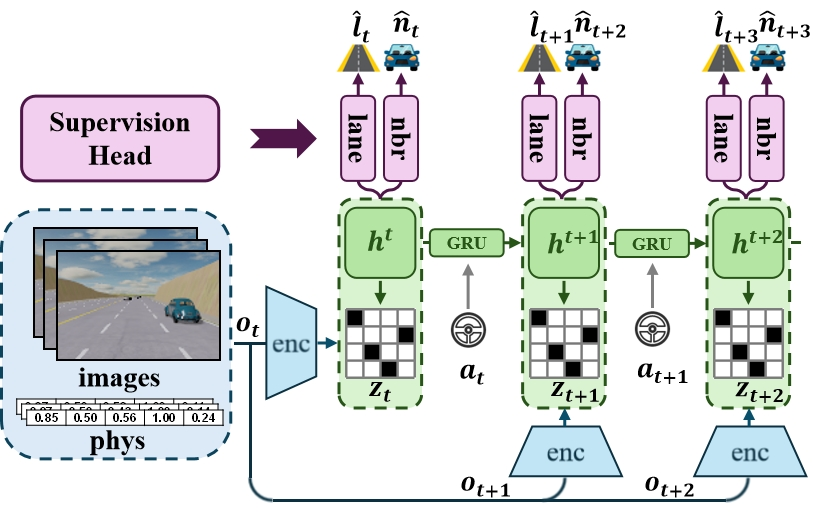
\includegraphics[width=1.0\columnwidth]{figures/world_model_learning2.png}  
    \caption{World Model Learning. The network encodes multi-modal inputs into latent states and decodes multiple task-specific outputs including reconstruction, prediction, and driving-aware supervision signals.} 
    \label{fig:world_model_learning} 
\end{figure}

\subsection{Actor-Critic learning}
Same as DreamerV3~\cite{hafner2025mastering}, we train an actor network $\pi(a \mid \phi)$ and critic network $V(\phi)$ using imagined trajectories:

The critic estimates state values using $\lambda$-returns:
\begin{equation}
\mathcal{L}_{\text{critic}} = \mathbb{E}_{\tau^{\text{imag}}} \left[ \sum_{\tau=t}^{t+H-1} \frac{1}{2} \left( V(\phi_\tau) - R_\tau^\lambda \right)^2 \right],
\end{equation}
with the $\lambda$-return defined as:
\begin{equation}
R_\tau^\lambda = r_\tau + \gamma \left[ (1-\lambda) v_\psi(s_{\tau+1}) + \lambda R_{\tau+1}^\lambda \right],
\end{equation}
where $\gamma$ is the discount factor, $\lambda \in [0,1]$ is the trace decay parameter, $r_\tau$ is the immediate reward, $v_\psi(s_{\tau+1})$ is the bootstrap value estimate from the target network, and $H$ denotes the length of imagined trajectories. Intuitively, $\lambda$-return considers cumulative rewards within finite-length imagined trajectories, while using $v_\psi(s_n)$ at the endpoint to approximate future returns infinitely far ahead, thereby providing a global value estimate for each state.

We adopt the dynamics gradient mode, which directly maximizes the value function along the imagined trajectory. The actor loss is defined as the negative expected advantage, weighted by the cumulative product of discounts and continuation probabilities:
\begin{equation}
\mathcal{L}_{\text{actor}} = -\mathbb{E}_{\tau^{\text{imag}}} \left[ \sum_{\tau=t}^{t+H-1} w_{\tau} \cdot \left( R_\tau^\lambda - V(\phi_{\tau}) \right) \right],
\label{eq:actor_loss}
\end{equation}
where $w_{\tau} = \gamma^{\tau-t} \prod_{k=t}^{\tau-1} c_{k}$ is the cumulative weight, $c_{k}$ is the predicted continuation probability from the continuation head.
\begin{figure}[htbp]
    \centering  
    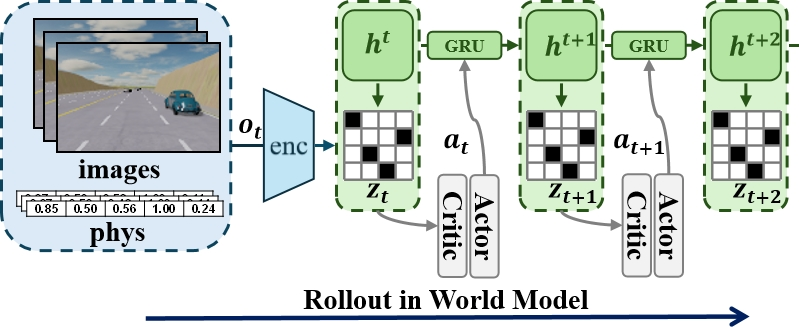
\includegraphics[width=1.0\columnwidth]{figures/actor_critic_learning.png}  
    \caption{Actor-Critic Learning. Imagined trajectories generated by the world model enable policy optimization in latent space. The actor predicts actions $\pi(a \mid \phi)$ while the critic estimates values $V(\phi)$ via $\lambda$-returns, allowing gradient-based updates without real environment interaction.} 
    \label{fig:actor_critic_learning} 
\end{figure}
\subsection{Reward Design}
The reward function $R$ in our driving task is composed of four components that balance progress, safety, and rule compliance:

The forward distance reward $R_1$ encourages making progress along the lane centerline:
\begin{equation}
R_1 = \beta_d \times (s_t - s_{t-1}) \times \mathbf{1}_{\text{pos}},
\end{equation}
where $s_t$ is the longitudinal projection of the vehicle onto the lane centerline, and $\mathbf{1}_{\text{pos}}$ indicates correct driving direction.

The speed reward $R_2$ encourages maintaining an appropriate speed:
\begin{equation}
R_2 = \beta_s \times (v / v_{\max}) \times \mathbf{1}_{\text{pos}},
\end{equation}
where $v$ is the current speed and $v_{\max}=80\,\mathrm{km/h}$.

The lane center offset penalty $R_3$ penalizes deviation from the lane center:
\begin{equation}
R_3 = -\beta_c \times (|y_t|) / w_{\text{lane}},
\end{equation}
where $y_t$ denotes lateral offset and $w_{\text{lane}}$ is lane width.

The termination reward/punishment $R_4$ provides a sparse terminal reward for completing the route or penalty for violations:
\begin{equation}
R_4 = 
\begin{cases}
r_{\text{success}} & \text{if episode completes successfully} \\
-p_{\text{crash}} & \text{if collision occurs} \\
-p_{\text{out}} & \text{if vehicle drives out of road} \\
\end{cases}.
\end{equation}

The total reward for each timestep is:
\begin{equation}
R = R_1 + R_2 + R_3 + R_4.
\end{equation}

\begin{algorithm}[t]
\caption{Kinematics-Aware World Model}
\label{alg:driveworld}
\begin{algorithmic}[1]
\Require environment, initial policy, hyperparameters
\Ensure trained policy
\State Initialize replay buffer $\mathcal{D}$
\State Initialize world model parameters $\theta$, actor parameters $\phi$, critic parameters $\psi$
\State Prefill $\mathcal{D}$ with random actions
\For{each iteration $k = 1, \dots, K$}
    \State Sample batch $\{(o_t, a_t, r_t)\}_{t=1}^{T}$ from $\mathcal{D}$
    \State \textcolor{gray}{\// World model learning}
    \State Encode $\mathbf{e}_t \leftarrow \textsc{Concat}\left(\textsc{CNN}(I_t; \theta_{\text{img}}), \textsc{MLP}(\mathbf{v}_t; \theta_{\text{phys}})\right)$
    \State Compute posterior and prior states via RSSM
    \State Compute losses: $\mathcal{L}_{\text{basic}}, \mathcal{L}_{\text{lane}}, \mathcal{L}_{\text{nbr}}$
    \State Update $\theta$ by minimizing total loss
    \State \textcolor{gray}{\// Behavior learning in imagination}
    \State Sample start states from posterior
    \State Generate imagined trajectory of length $H$ using actor and RSSM prior
    \State Compute $\lambda$-returns and advantages
    \State Update critic $\psi$ via regression to targets
    \State Update actor $\phi$ via dynamics gradient
    \State \textcolor{gray}{\// Environment interaction (parallel)}
    \State Rollout policy in environments for $N$ steps, adding to $\mathcal{D}$
\EndFor
\end{algorithmic}
\end{algorithm}